\documentclass[./main.tex]{subfiles}

\begin{document}
\section*{Appendix}

\begin{table}[htbp]
    \begin{adjustbox}{center}
        \begin{tabular}{c||ccc|ccc|ccc|ccc|c}
            \hline
            & \multicolumn{3}{c}{3DConv} & \multicolumn{3}{c}{DeciWatch} & \multicolumn{3}{c}{\begin{tabular}[c]{@{}c@{}}bi-ConvLSTM\\Model S\end{tabular}} & \multicolumn{3}{c}{\begin{tabular}[c]{@{}c@{}}bi-ConvLSTM\\Model C\end{tabular}} & Total \\ 
            \hline
            Experiment & 1.1 & 1.2 & 1.3 & 1.1 & 1.2 & 1.3 & 1.1 & 1.2 & 1.3 & 1.1 & 1.2 & 1.3 & \\
            \hline
            \hline
            Nose & 1.60 & 5.81 & 0.86 & 54.4 & 54.3 & 45.7 & 38.0 & 29.2 & 43.3 & 36.4 & 33.7 & 31.2 & 31.2 \\
            Ear & 1.34 & 4.99 & 0.71 & 54.8 & 54.8 & 46.3 & 40.3 & 33.5 & 35.6 & 36.8 & 37.3 & 33.9 & 31.7 \\
            Shoulder & 2.63 & 35.2 & 1.42 & 53.3 & 53.3 & 44.8 & 25.0 & 28.0 & 27.6 & 28.7 & 36.4 & 25.2 & 30.1 \\
            Elbow & 1.46 & 22.5 & 0.57 & 49.7 & 49.7 & 43.0 & 29.9 & 41.6 & 27.3 & 29.3 & 30.6 & 46.9 & 31.0 \\
            Wrist & 0.65 & 2.69 & 0.22 & 48.7 & 48.7 & 43.1 & 32.3 & 32.5 & 28.0 & 27.4 & 31.9 & 37.6 & 27.8 \\
            Hip & 3.64 & 58.1 & 0.93 & 49.8 & 49.8 & 43.0 & 28.0 & 24.9 & 16.6 & 25.1 & 23.5 & 16.3 & 28.3 \\
            Knee & 2.66 & 23.8 & 0.61 & 47.7 & 47.7 & 42.3 & 32.4 & 27.7 & 24.2 & 22.5 & 28.1 & 28.5 & 27.3 \\
            Ankle & 0.62 & 2.21 & 0.09 & 48.0 & 48.0 & 42.9 & 46.9 & 30.2 & 28.1 & 33.2 & 33.2 & 34.4 & 29.0 \\
            \hline
            Total & 1.84 & 20.5 & 0.67 & 51.4 & 51.4 & 44.5 & 27.8 & 31.1 & 33.8 & 29.5 & 31.7 & 31.8 & \\
            \hline
        \end{tabular}
    \end{adjustbox}
    \caption{Keypoint-specific testing PCK@0.05-accuracies of the various models for shifting-scalar $s = 1$. All the accuracies are in percentage.}
    \label{tab:pretrain_kpts_test_accs_05_1}
\end{table}

\begin{table}[htbp]
    \begin{adjustbox}{center}
        \begin{tabular}{c||ccc|ccc|ccc|ccc|c}
            \hline
            & \multicolumn{3}{c}{3DConv} & \multicolumn{3}{c}{DeciWatch} & \multicolumn{3}{c}{\begin{tabular}[c]{@{}c@{}}bi-ConvLSTM\\Model S\end{tabular}} & \multicolumn{3}{c}{\begin{tabular}[c]{@{}c@{}}bi-ConvLSTM\\Model C\end{tabular}} & Total \\ 
            \hline
            Experiment & 1.1 & 1.2 & 1.3 & 1.1 & 1.2 & 1.3 & 1.1 & 1.2 & 1.3 & 1.1 & 1.2 & 1.3 & \\
            \hline
            \hline
            Nose & 0.54 & 0.92 & 0.12 & 54.0 & 6.09 & 20.1 & 41.8 & 13.8 & 11.5 & 12.7 & 14.5 & 6.67 & 15.2 \\
            Ear & 0.75 & 2.40 & 0.23 & 53.6 & 5.11 & 20.2 & 47.9 & 20.5 & 15.9 & 21.7 & 21.6 & 15.6 & 18.8 \\
            Shoulder & 1.5 & 3.10 & 0.19 & 53.3 & 3.59 & 6.63 & 32.2 & 6.28 & 6.68 & 9.52 & 10.4 & 5.25 & 11.6 \\
            Elbow & 1.01 & 4.26 & 0.12 & 49.7 & 4.03 & 6.29 & 19.3 & 11.9 & 5.56 & 9.10 & 10.9 & 10.7 & 11.1 \\
            Wrist & 0.38 & 1.37 & 0.06 & 48.6 & 12.6 & 14.1 & 35.5 & 14.3 & 12.5 & 12.7 & 12.1 & 12.4 & 14.7 \\
            Hip & 1.36 & 3.42 & 0.12 & 49.8 & 4.68 & 3.99 & 19.9 & 6.76 & 11.4 & 7.66 & 6.43 & 7.87 & 10.3 \\
            Knee & 0.82 & 2.04 & 0.03 & 47.7 & 7.53 & 5.50 & 23.4 & 8.16 & 2.90 & 7.74 & 6.40 & 3.21 & 9.6 \\
            Ankle & 0.25 & 0.97 & 0.02 & 47.7 & 35.0 & 12.9 & 35.6 & 12.4 & 15.8 & 19.6 & 15.6 & 14.2 & 17.5 \\
            \hline
            Total & 0.80 & 2.40 & 0.11 & 51.2 & 51.2 & 10.3 & 10.5 & 11.6 & 10.1 & 12.5 & 12.0 & 9.63 & \\
            \hline
        \end{tabular}
    \end{adjustbox}
    \caption{Keypoint-specific testing PCK@0.05-accuracies of the various models for shifting-scalar $s = 2$. All the accuracies are in percentage.}
    \label{tab:pretrain_kpts_test_accs_05_2}
\end{table}

\begin{table}[htbp]
    \begin{adjustbox}{center}
        \begin{tabular}{c||ccc|ccc|ccc|ccc|c}
            \hline
            & \multicolumn{3}{c}{3DConv} & \multicolumn{3}{c}{DeciWatch} & \multicolumn{3}{c}{\begin{tabular}[c]{@{}c@{}}bi-ConvLSTM\\Model S\end{tabular}} & \multicolumn{3}{c}{\begin{tabular}[c]{@{}c@{}}bi-ConvLSTM\\Model C\end{tabular}} & Total \\ 
            \hline
            Experiment & 1.1 & 1.2 & 1.3 & 1.1 & 1.2 & 1.3 & 1.1 & 1.2 & 1.3 & 1.1 & 1.2 & 1.3 & \\
            \hline
            \hline
            Nose & 96.2 & 97.3 & 96.3 & 83.0 & 83.0 & 68.0 & 97.3 & 94.2 & 97.8 & 96.2 & 96.4 & 95.9 & 91.8 \\
            Ear & 96.3 & 97.0 & 96.3 & 85.1 & 85.1 & 70.0 & 96.8 & 96.3 & 96.9 & 96.3 & 96.4 & 96.1 & 92.4 \\
            Shoulder & 96.7 & 98.6 & 96.7 & 83.8 & 83.8 & 68.6 & 97.0 & 96.9 & 96.0 & 96.5 & 97.0 & 97.2 & 92.4 \\
            Elbow & 96.7 & 98.7 & 96.4 & 78.3 & 78.3 & 61.8 & 96.1 & 97.6 & 97.6 & 96.1 & 96.5 & 98.5 & 91.1 \\
            Wrist & 96.5 & 97.8 & 96.2 & 74.0 & 74.0 & 57.7 & 95.8 & 95.0 & 96.2 & 95.9 & 95.5 & 97.0 & 89.3 \\
            Hip & 96.8 & 99.1 & 96.3 & 80.3 & 80.3 & 64.0 & 93.5 & 95.7 & 96.6 & 96.8 & 95.3 & 96.3 & 90.1 \\
            Knee & 96.8 & 98.5 & 96.4 & 75.9 & 75.9 & 60.0 & 95.2 & 96.0 & 96.7 & 95.4 & 96.4 & 97.6 & 90.1 \\
            Ankle & 96.2 & 96.9 & 95.8 & 72.8 & 72.8 & 57.9 & 95.1 & 94.1 & 96.7 & 95.7 & 95.6 & 96.4 & 88.8 \\
            \hline
            Total & 96.6 & 98.0 & 96.3 & 80.2 & 80.2 & 64.2 & 95.7 & 95.8 & 96.7 & 96.1 & 96.1 & 96.9 & \\
            \hline
        \end{tabular}
    \end{adjustbox}
    \caption{Keypoint-specific testing PCK@0.2-accuracies of the various models for shifting-scalar $s = 1$. All the accuracies are in percentage.}
    \label{tab:pretrain_kpts_test_accs_20_1}
\end{table}

\begin{table}[htbp]
    \begin{adjustbox}{center}
        \begin{tabular}{c||ccc|ccc|ccc|ccc|c}
            \hline
            & \multicolumn{3}{c}{3DConv} & \multicolumn{3}{c}{DeciWatch} & \multicolumn{3}{c}{\begin{tabular}[c]{@{}c@{}}bi-ConvLSTM\\Model S\end{tabular}} & \multicolumn{3}{c}{\begin{tabular}[c]{@{}c@{}}bi-ConvLSTM\\Model C\end{tabular}} & Total \\ 
            \hline
            Experiment & 2.1 & 2.2 & 2.3 & 2.1 & 2.2 & 2.3 & 2.1 & 2.2 & 2.3 & 2.1 & 2.2 & 2.3 & \\
            \hline
            \hline
            Nose & 92.5 & 84.5 & 94.4 & 82.9 & 82.9 & 53.3 & 75.8 & 70.6 & 73.5 & 73.9 & 72.2 & 73.7 & 77.5 \\
            Ear & 92.0 & 91.1 & 94.4 & 85.0 & 85.0 & 51.0 & 80.3 & 77.7 & 77.7 & 80.8 & 79.2 & 79.9 & 81.2 \\
            Shoulder & 93.7 & 91.9 & 95.6 & 83.8 & 83.8 & 40.8 & 74.7 & 68.2 & 68.9 & 70.4 & 68.1 & 68.3 & 75.7 \\
            Elbow & 94.8 & 92.3 & 95.8 & 78.3 & 78.3 & 39.9 & 58.2 & 66.7 & 64.7 & 67.0 & 61.6 & 63.3 & 71.7 \\
            Wrist & 94.8 & 92.6 & 96.0 & 73.9 & 74.0 & 56.0 & 69.4 & 66.3 & 69.4 & 75.6 & 65.4 & 69.4 & 75.2 \\
            Hip & 94.5 & 91.6 & 95.7 & 80.3 & 80.3 & 46.0 & 64.7 & 61.9 & 67.5 & 80.7 & 57.3 & 74.8 & 74.6 \\
            Knee & 95.0 & 92.7 & 95.7 & 75.9 & 75.9 & 53.3 & 60.1 & 65.9 & 64.7 & 68.6 & 57.0 & 54.5 & 71.6 \\
            Ankle & 95.2 & 94.1 & 95.6 & 72.7 & 72.7 & 57.7 & 69.4 & 67.3 & 72.5 & 78.1 & 67.5 & 77.5 & 76.7 \\
            \hline
            Total & 94.2 & 91.8 & 95.5 & 80.2 & 80.2 & 50.3 & 68.5 & 67.8 & 69.6 & 74.6 & 65.5 & 70.0 & \\
            \hline
        \end{tabular}
    \end{adjustbox}
    \caption{Keypoint-specific testing PCK@0.2-accuracies of the various models for shifting-scalar $s = 2$. All the accuracies are in percentage.}
    \label{tab:pretrain_kpts_test_accs_20_2}
\end{table}

\begin{table}[htbp]
    \begin{adjustbox}{center}
        \begin{tabular}{c||ccc|ccc|ccc|ccc|c}
            \hline
            & \multicolumn{3}{c}{3DConv} & \multicolumn{3}{c}{DeciWatch} & \multicolumn{3}{c}{\begin{tabular}[c]{@{}c@{}}bi-ConvLSTM\\ Model S\end{tabular}} & \multicolumn{3}{c}{\begin{tabular}[c]{@{}c@{}}bi-ConvLSTM\\ Model C\end{tabular}} & Total \\ 
            \hline
            Experiment & 1.1 & 1.2 & 1.3 & 1.1 & 1.2 & 1.3 & 1.1 & 1.2 & 1.3 & 1.1 & 1.2 & 1.3 & \\
            \hline
            \hline
            Nose & 38.6 & 50.1 & 44.5 & 76.8 & 76.7 & 68.3 & 51.2 & 23.2 & 34.7 & 31.0 & 23.1 & 26.7 & 45.4 \\
            Ear & 33.4 & 40.3 & 37.4 & 77.3 & 77.2 & 69.1 & 40.0 & 28.5 & 35.9 & 44.3 & 31.1 & 55.3 & 47.5 \\
            Shoulder & 51.4 & 62.1 & 59.9 & 77.5 & 77.7 & 69.7 & 42.0 & 34.8 & 28.6 & 34.6 & 45.6 & 33.0 & 51.4 \\
            Elbow & 61.5 & 60.8 & 62.3 & 76.7 & 76.8 & 67.4 & 39.5 & 24.2 & 36.0 & 38.9 & 47.1 & 50.7 & 53.5 \\
            Wrist & 44.0 & 46.5 & 44.7 & 75.9 & 75.9 & 67.0 & 30.4 & 34.1 & 40.0 & 34.9 & 39.5 & 52.4 & 48.8 \\
            Pinky & 30.5 & 29.1 & 27.4 & 73.9 & 74.1 & 65.7 & 19.6 & 28.9 & 32.0 & 15.8 & 20.5 & 24.7 & 36.9 \\
            Index finger & 39.1 & 38.9 & 40.4 & 74.6 & 75.0 & 66.4 & 32.4 & 33.0 & 40.8 & 34.0 & 40.3 & 34.3 & 45.8 \\
            Thumb & 35.7 & 35.8 & 36.7 & 74.8 & 74.7 & 66.1 & 21.6 & 36.3 & 33.3 & 29.5 & 25.0 & 24.8 & 41.2 \\
            Hip & 79.3 & 76.9 & 87.2 & 79.9 & 80.2 & 71.3 & 45.4 & 50.8 & 51.9 & 42.9 & 50.4 & 40.8 & 63.1 \\
            Knee & 54.3 & 61.2 & 53.6 & 77.8 & 78.0 & 69.0 & 35.0 & 33.8 & 47.4 & 31.6 & 30.8 & 26.8 & 49.9 \\
            Ankle & 51.2 & 57.6 & 55.5 & 78.7 & 78.9 & 67.8 & 49.9 & 43.7 & 43.5 & 50.2 & 57.2 & 40.8 & 56.3 \\
            Heel & 64.4 & 62.8 & 69.0 & 77.9 & 77.5 & 67.0 & 34.3 & 33.3 & 38.0 & 37.8 & 36.5 & 36.2 & 52.9 \\
            Toes & 57.9 & 57.0 & 61.2 & 76.4 & 76.4 & 68.6 & 57.2 & 43.8 & 44.0 & 40.7 & 51.6 & 53.0 & 57.3 \\
            \hline
            Total & 49.7 & 52.3 & 53.1 & 76.6 & 76.7 & 68.1 & 37.8 & 34.9 & 39.0 & 35.9 & 39.0 & 38.5 & \\
            \hline
        \end{tabular}
    \end{adjustbox}
    \caption{Keypoint-specific testing PCK@0.05-accuracies of the various models for shifting-scalar $s = 1$. All the accuracies are in percentage.}
    \label{tab:finetune_kpts_test_accs_05_1}
\end{table}

\begin{table}[htbp]
    \begin{adjustbox}{center}
        \begin{tabular}{c||ccc|ccc|ccc|ccc|c}
            \hline
            & \multicolumn{3}{c}{3DConv} & \multicolumn{3}{c}{DeciWatch} & \multicolumn{3}{c}{\begin{tabular}[c]{@{}c@{}}bi-ConvLSTM\\ Model S\end{tabular}} & \multicolumn{3}{c}{\begin{tabular}[c]{@{}c@{}}bi-ConvLSTM\\ Model C\end{tabular}} & Total \\ 
            \hline
            Experiment & 1.1 & 1.2 & 1.3 & 1.1 & 1.2 & 1.3 & 1.1 & 1.2 & 1.3 & 1.1 & 1.2 & 1.3 & \\
            \hline
            \hline
            Nose & 33.0 & 49.3 & 37.7 & 74.3 & 74.5 & 22.4 & 33.1 & 32.3 & 36.0 & 22.6 & 27.4 & 30.7 & 39.4 \\
            Ear & 30.8 & 35.1 & 30.3 & 72.9 & 72.9 & 43.8 & 36.4 & 33.2 & 40.2 & 29.7 & 37.1 & 45.8 & 42.4 \\
            Shoulder & 48.7 & 56.6 & 51.5 & 77.0 & 77.0 & 31.0 & 49.9 & 45.3 & 27.0 & 40.2 & 41.5 & 37.9 & 48.6 \\
            Elbow & 56.8 & 58.8 & 54.4 & 76.6 & 76.6 & 30.2 & 34.2 & 47.8 & 37.1 & 54.8 & 45.6 & 32.6 & 50.5 \\
            Wrist & 43.5 & 46.0 & 41.2 & 74.7 & 74.7 & 36.3 & 25.6 & 35.2 & 40.0 & 34.1 & 40.7 & 39.6 & 44.3 \\
            Pinky & 28.6 & 29.5 & 28.2 & 73.6 & 74.0 & 30.6 & 27.5 & 20.6 & 28.0 & 21.2 & 24.8 & 31.3 & 34.8 \\
            Index finger & 39.3 & 40.7 & 40.7 & 74.8 & 74.5 & 30.6 & 42.2 & 33.4 & 44.7 & 37.7 & 30.3 & 38.2 & 43.9 \\
            Thumb & 36.0 & 35.3 & 36.6 & 74.9 & 74.4 & 28.1 & 28.1 & 28.5 & 16.1 & 24.2 & 24.3 & 24.6 & 35.9 \\
            Hip & 78.2 & 75.7 & 82.6 & 80.0 & 80.1 & 42.7 & 55.3 & 27.6 & 53.9 & 53.9 & 59.9 & 8.22 & 58.2 \\
            Knee & 39.7 & 57.5 & 37.5 & 78.3 & 78.1 & 24.8 & 44.8 & 26.1 & 17.4 & 47.1 & 42.8 & 50.7 & 45.4 \\
            Ankle & 37.2 & 62.9 & 39.4 & 75.8 & 76.0 & 53.9 & 46.3 & 46.1 & 34.9 & 51.2 & 49.2 & 45.7 & 51.6 \\
            Heel & 65.3 & 60.3 & 68.8 & 78.2 & 77.8 & 55.1 & 24.3 & 32.8 & 40.1 & 42.5 & 29.4 & 37.7 & 51.0 \\
            Toes & 61.4 & 62.4 & 60.0 & 75.8 & 75.9 & 32.8 & 54.1 & 72.1 & 42.1 & 39.1 & 53.0 & 56.0 & 57.1 \\
            \hline
            Total & 46.5 & 51.6 & 47.3 & 76.0 & 75.9 & 36.8 & 38.8 & 37.4 & 35.9 & 39.2 & 39.5 & 37.1 & \\
            \hline
        \end{tabular}
    \end{adjustbox}
    \caption{Keypoint-specific testing PCK@0.05-accuracies of the various models for shifting-scalar $s = 2$. All the accuracies are in percentage.}
    \label{tab:finetune_kpts_test_accs_05_2}
\end{table}

\begin{table}[htbp]
    \begin{adjustbox}{center}
        \begin{tabular}{c||ccc|ccc|ccc|ccc|c}
            \hline
            & \multicolumn{3}{c}{3DConv} & \multicolumn{3}{c}{DeciWatch} & \multicolumn{3}{c}{\begin{tabular}[c]{@{}c@{}}bi-ConvLSTM\\ Model S\end{tabular}} & \multicolumn{3}{c}{\begin{tabular}[c]{@{}c@{}}bi-ConvLSTM\\ Model C\end{tabular}} & Total \\ 
            \hline
            Experiment & 1.1 & 1.2 & 1.3 & 1.1 & 1.2 & 1.3 & 1.1 & 1.2 & 1.3 & 1.1 & 1.2 & 1.3 & \\
            \hline
            \hline
            Nose & 100 & 100 & 100 & 99.8 & 99.8 & 99.8 & 100 & 100 & 99.9 & 100 & 99.7 & 99.9 & 99.9 \\
            Ear & 100 & 100 & 100 & 99.8 & 99.8 & 99.8 & 97.7 & 99.9 & 100 & 100 & 100 & 99.9 & 99.7 \\
            Shoulder & 99.9 & 100 & 99.9 & 99.8 & 99.8 & 99.8 & 100 & 100 & 99.9 & 100 & 100 & 100 & 99.9 \\
            Elbow & 99.9 & 99.9 & 99.9 & 99.4 & 99.4 & 99.4 & 100 & 100 & 100 & 100 & 99.9 & 100 & 99.8 \\
            Wrist & 99.8 & 99.9 & 99.9 & 99.1 & 99.2 & 99.1 & 100 & 99.9 & 99.8 & 100 & 99.9 & 100 & 99.7 \\
            Pinky & 93.4 & 93.1 & 94.4 & 98.3 & 98.4 & 98.3 & 97.2 & 98.8 & 97.0 & 98.0 & 99.0 & 98.6 & 97.0 \\
            Index finger & 99.0 & 98.8 & 98.8 & 98.2 & 98.2 & 98.2 & 99.5 & 98.7 & 97.0 & 99.6 & 99.4 & 99.4 & 98.7 \\
            Thumb & 98.9 & 98.8 & 98.9 & 98.3 & 98.3 & 98.3 & 96.8 & 99.6 & 97.8 & 99.7 & 98.6 & 99.6 & 98.6 \\
            Hip & 99.9 & 100 & 100 & 99.7 & 99.7 & 99.7 & 100 & 100 & 100 & 100 & 100 & 100 & 99.9 \\
            Knee & 100 & 100 & 99.9 & 99.7 & 99.7 & 99.7 & 100 & 100 & 100 & 100 & 100 & 100 & 99.9 \\
            Ankle & 100 & 100 & 100 & 99.5 & 99.5 & 99.5 & 100 & 100 & 99.9 & 100 & 100 & 99.9 & 99.9 \\
            Heel & 100 & 100 & 100 & 99.2 & 99.2 & 99.2 & 99.3 & 99.9 & 99.9 & 99.9 & 100 & 99.8 & 99.7 \\
            Toes & 99.9 & 100 & 100 & 99.1 & 99.0 & 99.1 & 99.6 & 99.8 & 99.4 & 99.8 & 100 & 99.8 & 99.6 \\
            \hline
            Total & 99.2 & 99.3 & 99.3 & 99.2 & 99.2 & 96.1 & 99.4 & 99.7 & 99.2 & 99.8 & 99.7 & 99.7 & \\
            \hline
        \end{tabular}
    \end{adjustbox}
    \caption{Keypoint-specific testing PCK@0.2-accuracies of the various models for shifting-scalar $s = 1$. All the accuracies are in percentage.}
    \label{tab:finetune_kpts_test_accs_2_1}
\end{table}

\begin{table}[htbp]
    \begin{adjustbox}{center}
        \begin{tabular}{c||ccc|ccc|ccc|ccc|c}
            \hline
            & \multicolumn{3}{c}{3DConv} & \multicolumn{3}{c}{DeciWatch} & \multicolumn{3}{c}{\begin{tabular}[c]{@{}c@{}}bi-ConvLSTM\\ Model S\end{tabular}} & \multicolumn{3}{c}{\begin{tabular}[c]{@{}c@{}}bi-ConvLSTM\\ Model C\end{tabular}} & Total \\ 
            \hline
            Experiment & 2.1 & 2.2 & 2.3 & 2.1 & 2.2 & 2.3 & 2.1 & 2.2 & 2.3 & 2.1 & 2.2 & 2.3 & \\
            \hline
            \hline
            Nose & 100 & 100 & 100 & 99.8 & 99.8 & 97.2 & 100 & 99.9 & 99.7 & 99.7 & 99.9 & 100 & 99.7 \\
            Ear & 100 & 99.8 & 100 & 99.7 & 99.7 & 97.1 & 99.8 & 99.8 & 100 & 99.9 & 99.9 & 99.9 & 99.6 \\
            Shoulder & 99.9 & 99.7 & 99.9 & 99.8 & 99.9 & 95.8 & 99.9 & 99.8 & 100 & 99.9 & 100 & 100 & 99.6 \\
            Elbow & 99.8 & 99.9 & 99.9 & 99.5 & 99.4 & 90.8 & 100 & 99.5 & 100 & 100 & 100 & 100 & 99.1 \\
            Wrist & 99.8 & 100 & 99.9 & 99.1 & 99.1 & 94.4 & 99.8 & 99.7 & 99.8 & 99.8 & 100 & 99.7 & 99.3 \\
            Pinky & 93.1 & 93.7 & 93.9 & 98.4 & 98.4 & 86.5 & 97.7 & 98.0 & 97.9 & 99.1 & 96.0 & 98.2 & 95.9 \\
            Index finger & 98.9 & 99.0 & 98.8 & 98.2 & 98.2 & 88.9 & 99.4 & 99.1 & 99.2 & 99.6 & 98.0 & 97.5 & 97.9 \\
            Thumb & 98.6 & 98.6 & 98.6 & 98.3 & 98.2 & 90.1 & 95.7 & 96.6 & 98.6 & 97.5 & 98.3 & 99.6 & 97.4 \\
            Hip & 100 & 99.9 & 100 & 99.7 & 99.8 & 95.1 & 99.9 & 99.8 & 99.9 & 99.8 & 100 & 99.9 & 99.5 \\
            Knee & 100 & 100 & 99.9 & 99.6 & 99.7 & 95.1 & 100 & 99.9 & 99.9 & 99.9 & 99.9 & 100 & 99.5 \\
            Ankle & 100 & 99.9 & 100 & 99.5 & 99.5 & 93.9 & 100 & 100 & 100 & 100 & 100 & 100 & 99.4 \\
            Heel & 100 & 100 & 100 & 99.3 & 99.3 & 91.0 & 99.9 & 99.9 & 99.8 & 99.9 & 99.6 & 99.9 & 99.1 \\
            Toes & 99.9 & 100 & 100 & 99.0 & 99.1 & 91.9 & 99.9 & 99.4 & 98.4 & 99.8 & 99.6 & 99.8 & 98.9 \\
            \hline
            Total & 99.2 & 99.3 & 99.2 & 99.2 & 99.2 & 92.8 & 99.4 & 99.5 & 99.3 & 99.6 & 99.3 & 99.6 & \\
            \hline
        \end{tabular}
    \end{adjustbox}
    \caption{Keypoint-specific testing PCK@0.2-accuracies of the various models for shifting-scalar $s = 2$. All the accuracies are in percentage.}
    \label{tab:finetune_kpts_test_accs_2_2}
\end{table}


\begin{figure}[h]
    \centering
    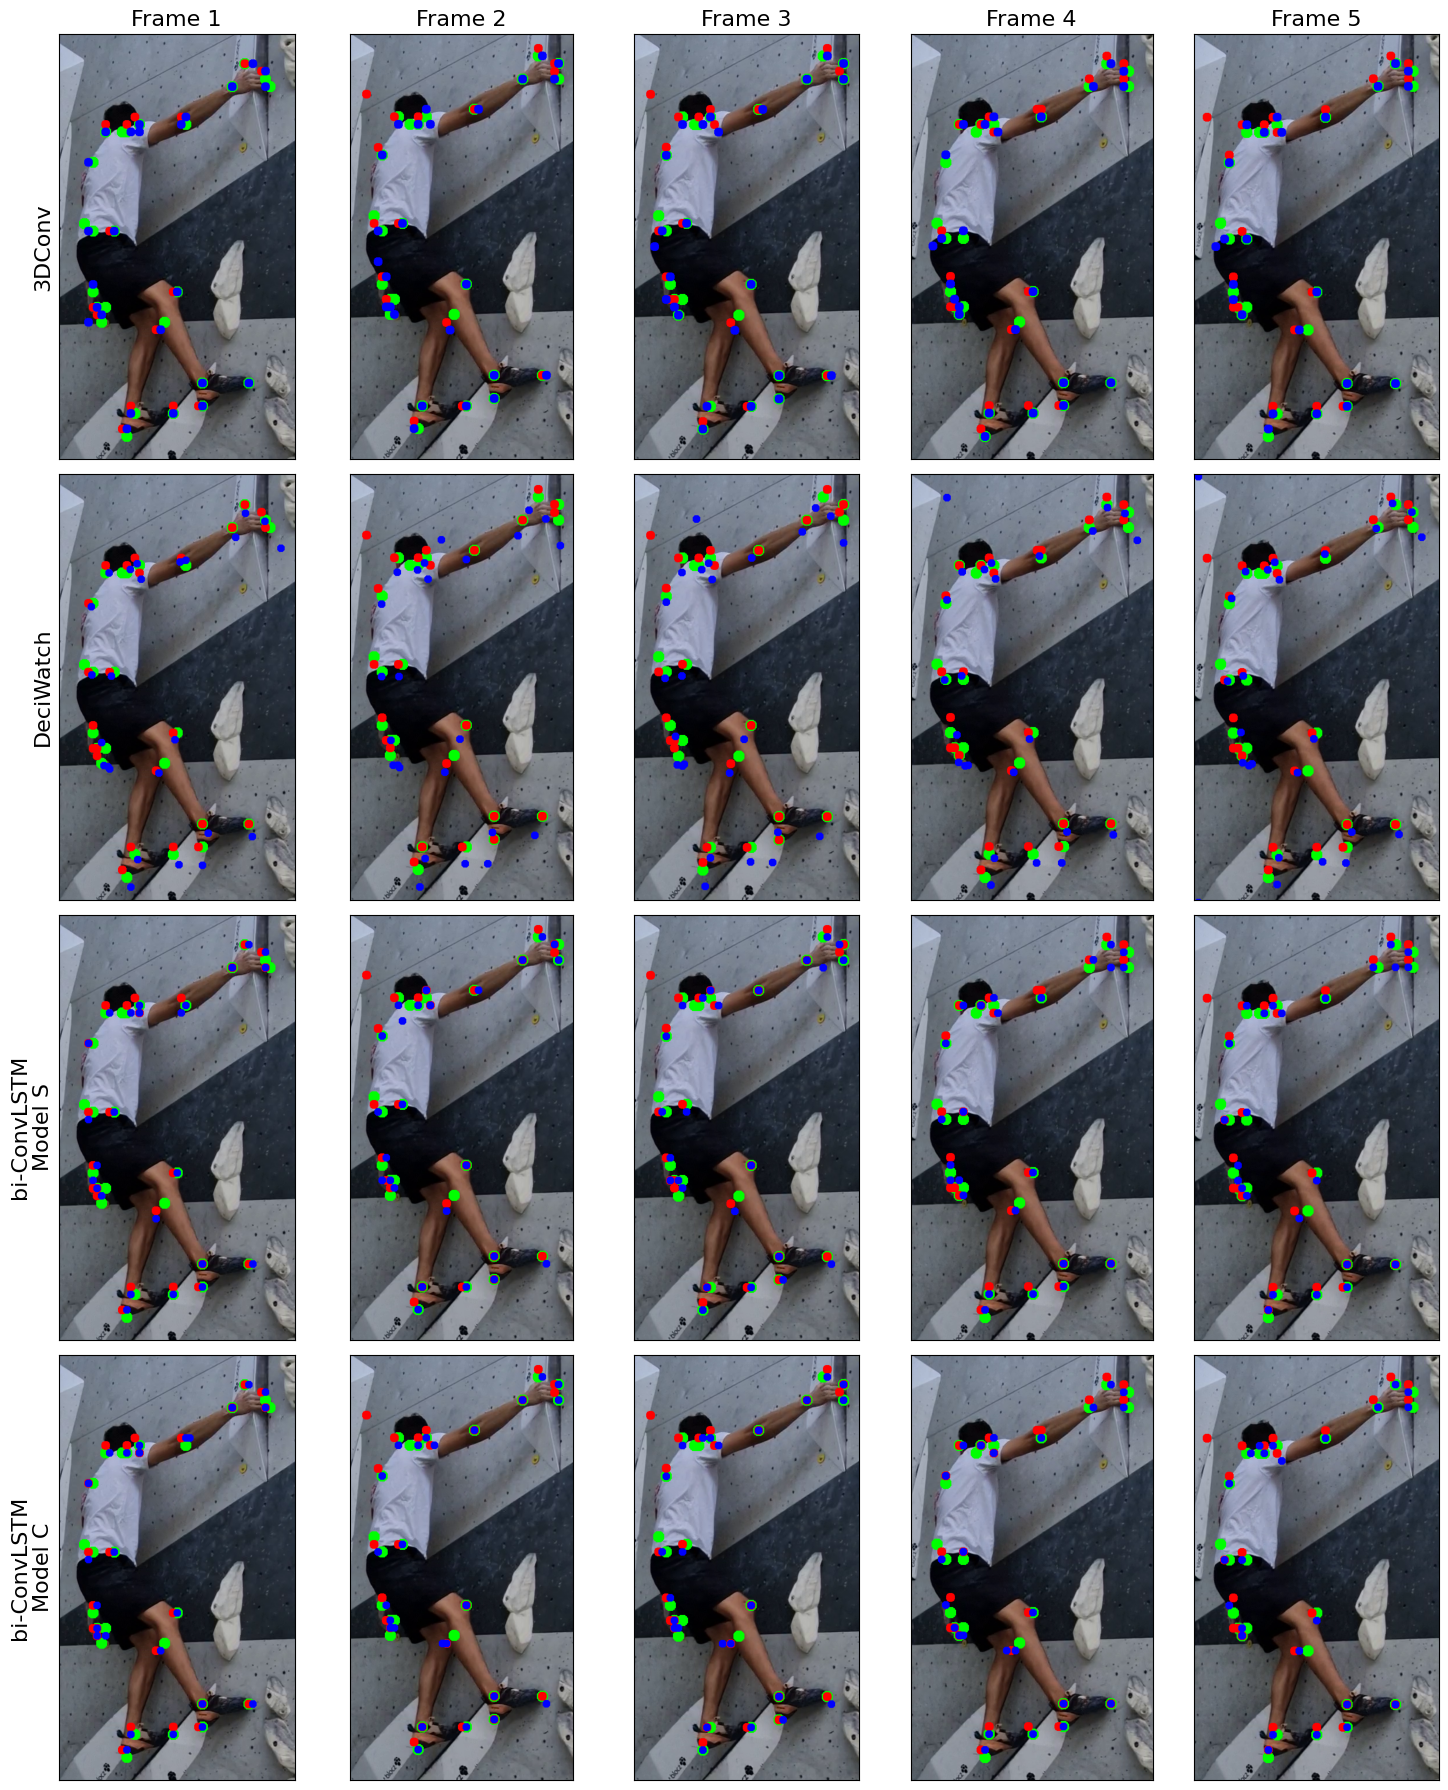
\includegraphics[width=0.95\textwidth]{./entities/predictions.png}
    \caption{Ground truth keypoints (green), Mask R-CNN predictions (red) and predictions of the best setting of each model from section \ref{subsec:finetune_test_res} on five consecutive frames from the single hold-out video.}
    \label{fig:predictions}
\end{figure}

\end{document}